\setAuthor{Eero Vaher}
\setRound{lahtine}
\setYear{2014}
\setNumber{G 4}
\setDifficulty{3}
\setTopic{Elektriahelad}

\prob{Tetraeeder}
Tetraeedri (neljast võrdkülgsest kolmnurgast koosneva püramiidi) servadeks on ühesugused takistid takistusega $R$. Leidke tetraeedri kahe tipu vaheline takistus.

\hint
Takistuse leidmiseks tasub tetraeedri pinna jaotus joonistada ning ära kasutada sümmeetriat.

\solu
Alloleval joonisel on toodud tetraeedri ekvivalentskeem. Sümmeetriakaalutlustel ei saa tippude C ja D vaheline takisti mõjutada tippude A ja B vahelist takistust, järelikult võib selle skeemilt eemaldada. Allesjääva skeemi takistust on lihtne leida.
\[R_\text{AB}=\left(\frac{1}{R+R}+\frac{1}{R+R}+\frac{1}{R}\right)^{-1}=\frac{R}{2}.\]
\begin{center}
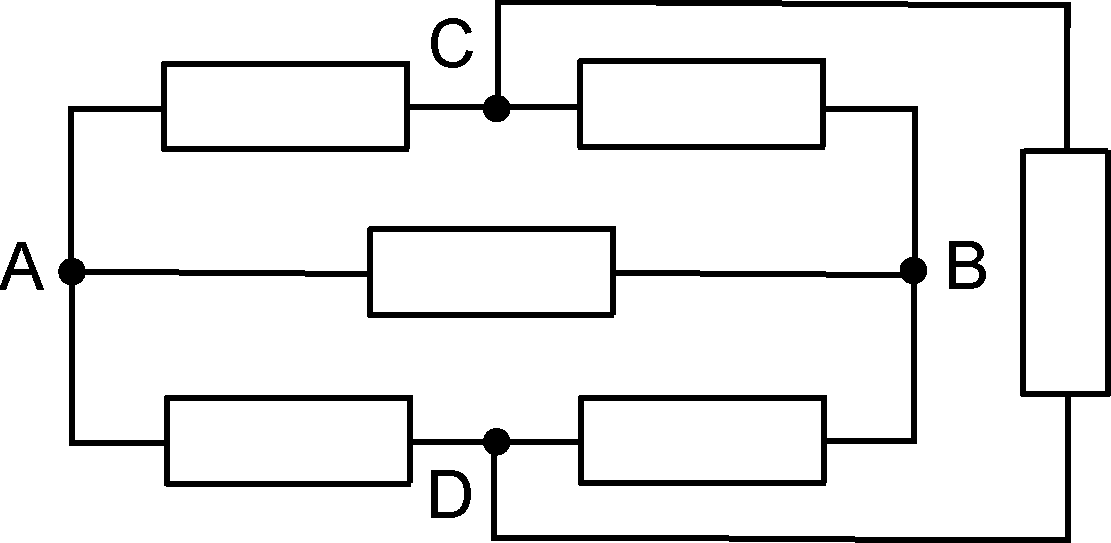
\includegraphics[width=0.6\linewidth]{2014-lahg-04-skeem}
\end{center}

\probeng{Tetrahedron}
A tetrahedron’s (a pyramid made of four equilateral triangles) edges are identical resistors with a resistance $R$. Find the resistance between the tetrahedron’s two tips.

\hinteng
To find the resistance you should sketch the surface development of the tetrahedron and make use of the symmetry.

\solueng
The equivalent diagram of the tetrahedron is pictured in the figure below. Based on symmetry considerations the resistance between the tips C and D cannot affect the resistance between the tips A and B, therefore we can remove that from the diagram. The resistance of the remaining diagram is easy to find.
\[R_\text{AB}=\left(\frac{1}{R+R}+\frac{1}{R+R}+\frac{1}{R}\right)^{-1}=\frac{R}{2}.\]
\begin{center}
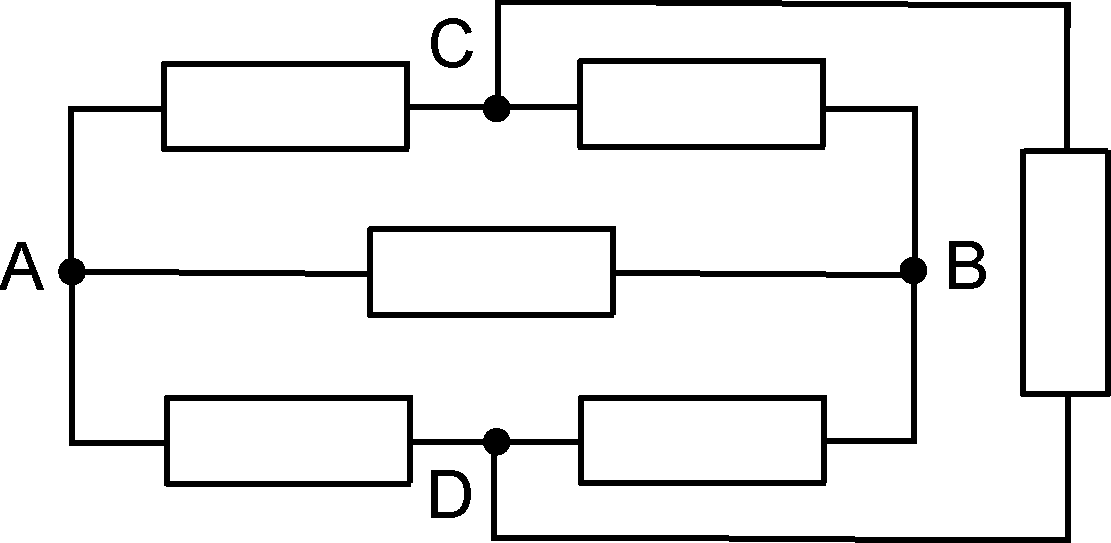
\includegraphics[width=0.6\linewidth]{2014-lahg-04-skeem}
\end{center}
\probend